%%%%%%%%%%%%%%%%%%%%%%%%%%%%%%%%%%%%%%%%%%%%%%%%%%%%%%%%%%%%%%%%%%%%%%%%%%%%%%%%%%%%%%%%%%%%%%%%%%%%%%%%%%%%%%%%%%%%%%%%%%%%%%%%%%%%%%%%%%%%%%%%%%%%%%%%%%%
% This is just an example/guide for you to refer to when submitting manuscripts to Frontiers, it is not mandatory to use Frontiers .cls files nor frontiers.tex  %
% This will only generate the Manuscript, the final article will be typeset by Frontiers after acceptance.   
%                                              %
%                                                                                                                                                         %
% When submitting your files, remember to upload this *tex file, the pdf generated with it, the *bib file (if bibliography is not within the *tex) and all the figures.
%%%%%%%%%%%%%%%%%%%%%%%%%%%%%%%%%%%%%%%%%%%%%%%%%%%%%%%%%%%%%%%%%%%%%%%%%%%%%%%%%%%%%%%%%%%%%%%%%%%%%%%%%%%%%%%%%%%%%%%%%%%%%%%%%%%%%%%%%%%%%%%%%%%%%%%%%%%

%%% Version 3.4 Generated 2022/06/14 %%%
%%% You will need to have the following packages installed: datetime, fmtcount, etoolbox, fcprefix, which are normally inlcuded in WinEdt. %%%
%%% In http://www.ctan.org/ you can find the packages and how to install them, if necessary. %%%
%%%  NB logo1.jpg is required in the path in order to correctly compile front page header %%%

\documentclass[utf8]{FrontiersinHarvard}

%\setcitestyle{square} % for Physics and Applied Mathematics and Statistics articles
\usepackage{url,hyperref,lineno,microtype,subcaption}
\usepackage[onehalfspacing]{setspace}

\linenumbers


% BELOW TAKEN FROM rticles plos template
%
% amsmath package, useful for mathematical formulas
\usepackage{amsmath}
% amssymb package, useful for mathematical symbols
\usepackage{amssymb}

% hyperref package, useful for hyperlinks
\usepackage{hyperref}

% graphicx package, useful for including eps and pdf graphics
% include graphics with the command \includegraphics
\usepackage{graphicx}

% Sweave(-like)
\usepackage{fancyvrb}
\DefineVerbatimEnvironment{Sinput}{Verbatim}{fontshape=sl}
\DefineVerbatimEnvironment{Soutput}{Verbatim}{}
\DefineVerbatimEnvironment{Scode}{Verbatim}{fontshape=sl}
\newenvironment{Schunk}{}{}
\DefineVerbatimEnvironment{Code}{Verbatim}{}
\DefineVerbatimEnvironment{CodeInput}{Verbatim}{fontshape=sl}
\DefineVerbatimEnvironment{CodeOutput}{Verbatim}{}
\newenvironment{CodeChunk}{}{}

% cite package, to clean up citations in the main text. Do not remove.
\usepackage{cite}

\usepackage{color}

% Below is from frontiers

% Leave a blank line between paragraphs instead of using \\


\def\keyFont{\fontsize{8}{11}\helveticabold }


%% ** EDIT HERE **
%% PLEASE INCLUDE ALL MACROS BELOW

%% END MACROS SECTION


% tightlist command for lists without linebreak
\providecommand{\tightlist}{%
  \setlength{\itemsep}{0pt}\setlength{\parskip}{0pt}}



\usepackage{booktabs}
\usepackage{longtable}
\usepackage{array}
\usepackage{multirow}
\usepackage{wrapfig}
\usepackage{float}
\usepackage{colortbl}
\usepackage{pdflscape}
\usepackage{tabu}
\usepackage{threeparttable}
\usepackage{threeparttablex}
\usepackage[normalem]{ulem}
\usepackage{makecell}
\usepackage{xcolor}

\def\Authors{
  Michael Schramm\,\textsuperscript{1*},
  Duncan Kikoyo\,\textsuperscript{1},
  Janelle Wright\,\textsuperscript{1},
  Shubham Jain\,\textsuperscript{1}}

\def\Address{

  \textsuperscript{1} Texas Water Resources Institute, Texas A\&M
AgriLife Research,  College Station,  Texas,  USA
  }

  \def\corrAuthor{Michael Schramm}\def\corrAddress{Texas Water Resources
Institute, Texas A\&M AgriLife Research\\1001 Holleman Dr E.\\College
Station, Texas, 77840 USA}\def\corrEmail{\href{mailto:michael.schramm@ag.tamu.edu}{\nolinkurl{michael.schramm@ag.tamu.edu}}}
  \def\firstAuthorLast{Schramm {et~al.}}
  
  
  
  
  
  


\begin{document}

\onecolumn
\firstpage{1}


\title[Meta-analysis of best management practices]{A meta-analysis of
the impacts of best management practices on nonpoint source pollutants.}
\author[\firstAuthorLast]{\Authors}
\address{} %This field will be automatically populated
\correspondance{} %This field will be automatically populated

\extraAuth{}% If there are more than 1 corresponding author, comment this line and uncomment the next one.
%\extraAuth{corresponding Author2 \\ Laboratory X2, Institute X2, Department X2, Organization X2, Street X2, City X2 , State XX2 (only USA, Canada and Australia), Zip Code2, X2 Country X2, email2@uni2.edu}


\maketitle

\begin{abstract}
Abstract length and content varies depending on article type. Refer to
\url{http://www.frontiersin.org/about/AuthorGuidelines} for abstract
requirement and length according to article type.

\tiny
 \keyFont{ \section{Keywords:} best management practice, water
quality, nonpoint source pollution, fecal indicator
bacteria, nutrients} %All article types: you may provide up to 8 keywords; at least 5 are mandatory.
\end{abstract}

\hypertarget{introduction}{%
\section{Introduction}\label{introduction}}

In the United States (U.S.), major progress towards water quality goals
have been achieved through the Clean Water Act of 1972. This progress
has been largely attributed to investments and reductions in point
source discharges while reductions in nonpoint source pollutants remain
a substantial challenge
\citep{benhamLessonsLearnedTMDL2008, nationalresearchcouncilAssessingTMDLApproach2001, schrammTotalMaximumDaily2022}.
Increased pollutant loads and pollutant concentrations in runoff are a
particular challenge when dealing with nonpoint source pollution
resulting from land use change. The impacts of land use change on
hydrology and water quality are well established
\citep{allanLandscapesRiverscapesInfluence2004, carpenterNonpointPollutionSurface1998, bernhardtUnderstandingManagingMinimizing2008, careyEvaluatingNutrientImpacts2013, freemanImpactsUrbanizationDevelopment2019}.
Nonpoint source driven fecal indicator bacteria (FIB), nitrogen,
phosphorus, and suspended sediment remain major causes of water quality
impairments in U.S. rivers and streams despite decades of work. In 2017,
the Environmental Protection Agency (EPA) estimated 41\% or more of the
nation's rivers and streams rated poorly for biological condition due to
excess nitrogen or phosphorus \citep{epaNationalWaterQuality2017}. FIB
remains the leading cause of water body impairment on the Clean Water
Act 303(d) list in the United States
\citep{epaNationalWaterQuality2017}.

Best management practices (BMPs) have been the primary suite of tools
for addressing nonpoint source pollution. BMPs are structural or
non-structural controls used to mitigate the effects of increased runoff
volume, pollutant loads, or pollutant concentrations emanating from
diffuse nonpoint sources. BMPs control the delivery of pollutants
through a few possible mechanisms. Structural BMPs reduce and retard
total volume of runoff, thus reducing both the volume of water and
pollutant load. Structural BMPs may also provide a mechanism for
physical, chemical, or biological removal of pollutant constituents
suspended or dissolved in runoff. Non-structural BMPs (such as nutrient
management or livestock management) are utilized to reduce the
generation of pollutant runoff by avoiding pollutant generation during
critical periods.

Practitioners rely extensively on mechanistic models to plan and
evaluate BMP scenarios and resulting water quality.
\citet{linternBestManagementPractices2020} found 43\% of reviewed BMP
effectiveness studies relied completely on modeled outputs, with modeled
outputs almost always predicting water quality improvements following
BMP implementation. However, field studies are much more likely to
demonstrate mixed results including net releases of pollutants under
certain conditions
\citep{linternBestManagementPractices2020, liuReviewEffectivenessBest2017}.
The disconnect between modeled outcomes and field studies might be
attributed to (1) overly simplified or incorrect estimates of parameters
that represent management practices
\citep{ullrichApplicationSoilWater2009, fuReviewCatchmentscaleWater2019, linternBestManagementPractices2020},
(2) failure to incorporate uncertainty in estimates
\citep{tasdighiBayesianTotalUncertainty2018, fuReviewCatchmentscaleWater2019, linternBestManagementPractices2020},
and (3) assumption of static performance over time
\citep{mealsLagTimeWater2010, liuReviewEffectivenessBest2017, fuReviewCatchmentscaleWater2019}.

A source of uncertainty comes from the substantial variability of
performance metrics reported in empirical BMP studies
\citep{linternBestManagementPractices2020}. Previous empirical reviews
generally describe high variability and uncertainty in nitrogen and
phosphorus removal and consistent reduction in total suspended sediment
concentrations across BMP types
\citep{linternBestManagementPractices2020, liuReviewEffectivenessBest2017, kochNitrogenRemovalStormwater2014, claryBMPPerformanceAnalysis2011, barrettComparisonBMPPerformance2008, grudzinskiDoesRiparianFencing2020}.
The review literature on the effects of BMPs on FIBs are sparse but
generally find extremely high variance in performance across BMPs
\citep{claryBMPPerformanceAnalysis2011, grudzinskiDoesRiparianFencing2020}.
Accurately characterizing BMP treated runoff quality is challenging due
to the high variability in BMP performance. However, influent water
quality, seasonality, and BMP age provide some explanatation to highliy
heterogenous BMP efficiency data
\citep{barrettPerformanceComparisonStructural2005, liuReviewEffectivenessBest2017}.\\
A recent meta-analysis demonstrated the further linkages between local
climatic conditions and BMP performance on nitrogen and phosphorus
concentrations \citep{horvathEffectsRegionalClimate2023}.

\hypertarget{methods}{%
\section{Methods}\label{methods}}

We conducted a systematic review of recent (2000-2022) literature to
compile field studies documenting the effectiveness of best management
practices on fecal indicator bacteria and nutrients concentrations. The
systematic review followed guidance provided in the Collaboration for
Environmental Evidence systematic review guidelines
\citep{collaborationforenvironmentalevidenceGuidelinesStandardsEvidence2018}.
In order to maximize the number of studies included in the review, we
included both peer-reviewed studies and unpublished white papers to
reduce potential bias against negative results. The inclusion criteria
filtered out (1) non-field studies, (2) modelling results, (3) studies
that did not evaluate specific BMPs, (4) studies conducted outside of
the U.S. or published in a language other than English. We ran search
queries in Texas A\&M Library Catalog, Web of Science, and Google
Scholar. Although results from Google Scholar are not always replicable,
we utilized the service to maximize search results for studies not
published in academic journals and presumably increase the chance of
identifying studies with negative effects. Fecal indicator bacteria
study seraches included the following query: ``fecal indicator
bacteria'' OR ``E. coli'' OR ``Escherichia coli'' OR ``enterococci'' OR
``enterococcus'' AND ``best management practices'' OR ``BMPs'' AND
``effectiveness'' OR ``performance''. Nutrient BMP studies utilized a
similar query: ``nutrient'' OR ``nitrogen'' OR ``phosphorus'' OR
``sediment'' OR ``TSS'' AND ``best management practices'' OR ``BMPs''
AND ``effectiveness'' OR ``performance''.

Results from each database were first filtered to remove duplicates.
After removal of duplicates, each member of the research team (\emph{n}
= 4) was assigned a subset of studies to evaluate if they should be
included. \textbf{include supplementary tables with inclusion criteria
and data variables} Each study was reviewed by two team members and
differences in opinion were collectively discussed and agreed upon
before progressing. The remaining studies were split among team members
for data extraction, again with at least two team members reviewing each
study. If data was provided in figures, the data was extracted with the
WebPlotDigitizer tool \citep{rohatgiWebPlotDigitizer2022}.

\begin{table}

\caption{\label{tab:criteria}Criteria applied for including or excluding studies within the review database.}
\centering
\begin{tabular}[t]{>{\raggedright\arraybackslash}p{5em}>{\raggedright\arraybackslash}p{15em}>{\raggedright\arraybackslash}p{15em}}
\toprule
Attribute & Inclusion Criteria & Excluision Criteria\\
\midrule
Study type & Journal articles, book chapters, conference papers, unpublished research reports, thesis and dissertations, organizational and agency white papers. & Synopsis or review studies, peports with reductions based on modeled or other estimated reductions (e.g. TMDLs, watershed plans, or modelling studies.\\
Outcomes & Field studies with measured effects on fecal indicator bacteria or nutrient concentrations. & Studies not explicitly linking reductions to a specific BMP or insufficient information to quantify reductions.\\
Geographical context & Studies conducted within the United States. & Studies outside of the United States.\\
Timeframe & Studies published from 2000 through 2022. & Studies published prior to 2000 or after 2022.\\
\bottomrule
\end{tabular}
\end{table}

\begin{table}

\caption{\label{tab:datvars}Study and effect variables extracted for review.}
\centering
\begin{tabular}[t]{>{\raggedright\arraybackslash}p{10em}>{\raggedright\arraybackslash}p{25em}}
\toprule
Variable & Description\\
\midrule
Publication Year & Year the study was published\\
Parameter & The specific pollutant measured.\\
Runoff source & Dominant source of runoff (rop fields, livestock pasture, commerical, residential\\
Source type & Major categorization of runoff source: agricultural or urban\\
BMP & BMP evaluated\\
\addlinespace
BMP Classification & BMP description based on NRCS conservation practice standards and EPA BMP fact sheets\\
BMP Category & BMP categorization based on structural or management\\
BMP Subcategory & BMP subcategorization based on pollutant removal processes\\
Study scale & Spatial scale of the study area ("lot/field", "community", "watershed")\\
Location & Location name used in the study description\\
\addlinespace
State & State where the study was conducted\\
Study area & Drainage area in hectares\\
Longitude & Approximated or reported latitude coordinate\\
Latitude & Approximated or reported longitude coordinate\\
Study years & Year or years when data were collected\\
\addlinespace
N control & Number of control measurements\\
N experiment & Number of experiemental measurements\\
X control & Mean concentration for control measurements\\
X experiment & Mean concentration for experiemental measurements\\
SE control & Standard error of control measurements\\
\addlinespace
SE experiment & Standard error of experimental measurements\\
Minimum control & Minimum control measurement\\
Minimum experiment & Minimum experiment measurement\\
Maximum control & Maximum control measurement\\
Maximum experiment & Maximum experiment measurement\\
\addlinespace
SD control & Standard deviation of control measreuments\\
SD experiment & Standard deviation of experimental measurements\\
Units & Units reported by the study\\
Percent reduction & BMP efficiency for studies that only reported efficiency\\
\bottomrule
\end{tabular}
\end{table}

\hypertarget{effect-size-calculation}{%
\subsection*{Effect size calculation}\label{effect-size-calculation}}
\addcontentsline{toc}{subsection}{Effect size calculation}

Prior BMP reviews routinely report the effect of BMPs using efficiency
values
\citep[see][]{agouridisLivestockGrazingManagement2005, krogerReviewBestManagement2012, liuEnhancingRainfallrunoffModel2015, simpsonDevelopingBestManagement2009}.
Efficiency values are calculated as:

\[
\text{Efficiency}=\frac{x_{control}-x_{experiment}}{x_{control}}\times 100,
\]

where \emph{x\textsubscript{control}} is the pre-treatment or control
pollutant concentration and \emph{x\textsubscript{experiment}} is the
pollutant concentration measured after the BMP intervention. There are
several statistical shortcomings (distributional asymetry, skewness, and
non-additive properties) when using efficiency to estimate overall
effect sizes
\citep{nuzzoPercentDifferencesAnother2018, coleStatisticsNotesWhat2017}.
In comparision, the log ratio of means (\emph{ROM}) provide preferable
statistical properties for regression analysis
\citep{osenbergEffectSizeEcological1997, hedgesMetaanalysisResponseRatios1999}.
\emph{ROM} quantifies the difference in means between the control and
experimental group \citep{hedgesMetaanalysisResponseRatios1999}:

\[
ROM_i = ln\left(\frac{x_{i,control}}{x_{i,experiment}}\right) = ln(x_{i, control})-ln(x_{i, experiment}),
\] where \emph{x\textsubscript{i,control}} and
\emph{x\textsubscript{i,experiment}} are the mean pollutant
concentrations for experiment \emph{i}. The statistical properties of
\emph{lnRR} (normal distribution around zero and additive properties)
are preferable to the more commonly reported efficiency metric
\citep{osenbergEffectSizeEcological1997, hedgesMetaanalysisResponseRatios1999}.
Use of \emph{ROM} required the exclusion of studies that only provided
measures of BMP efficiency and not the underlying data used to derive
the metric.

\hypertarget{statistical-models}{%
\subsection{Statistical models}\label{statistical-models}}

We used the ``rma.mv'' function in the \emph{metafor} R package to fit
multilevel random effects linear models with \emph{ROM} as the effect
variable
\citep{viechtbauerConductingMetaanalysesMetafor2010, rcoreteamLanguageEnvironmentStatistical2023}.
Our models specified a nested random effects term accounting for
heterogeneity between effect sizes from the same study and for
heterogeneity between studies. A key feature of meta-analysis is the
weighting of effects using sampling variance of individual effect sizes.
45\% of fecal indicator bacteria, 68\% of TN, 68\% of TP, and 70\% of
TSS effect sizes were missing standard deviations required to estimate
sampling variance. Removal of studies due to missing variance
information can introduce substantial bias
\citep{kambachConsequencesMultipleImputation2020}, so we imputed missing
standard deviations using random forest based multivariate imputation
with chained equations using the \emph{mice} R package
\citep{buurenMiceMultivariateImputation2011}. Sampling variance was
estimated with the variance estimator described in Doncaster et al.~to
reduce bias in small sample studies:

\[
v(ROM) = \frac{\sum_{i=1}^{K}{(CV^2_{control,i})/K}}{n_{control}} + \frac{\sum_{i=1}^{K}{(CV^2_{experiment,i})/K}}{n_{experiment}},
\]

where \emph{v} represents the sampling variance, \(CV_{control,i}\) and
\(CV^2_{experiment,i}\) are the coefficients of variation from the
\emph{i}th study for studies 1, 2, \ldots, \emph{K}.

Our initial models included log transformed pre-treatment pollutant
concentration, study scale (plot/field, community, watershed), study
length (\emph{n} years), BMP subcategory (), and pollutant
concentration:BMP subcategory interactions were included as fixed effect
terms. We used an information-theoretic approach to select the most
parsimonious model from the subset of candidate models based on
corrected Akaike information criterion (AIC\textsubscript{c}) estimated
with maximum likelihood \citep{cinarUsingInformationTheoretic2021}. The
final model was selected from candidate models, which included all
combination and subsets of the full model, by eliminating candidate
models until the \(\Delta\)\emph{AIC\textsubscript{c}} reached \(\leq\)
2 \citep{burnhamAICModelSelection2011}. We estimated regression
coefficients of the selected model using restricted maximum likelihood.
Relative heterogeneity between and within studies were calculated using
the \emph{I\textsuperscript{2}} metric described in
\citet{nakagawaMethodologicalIssuesAdvances2012}. Marginal
\emph{R\textsuperscript{2}} was used to describe the amount of variance
explained by fixed effects \citep{nakagawaGeneralSimpleMethod2013}.

We tested for evidence of publication bias, in the form of small study
effect, by using the extension of Egger's regression applied to the
multilevel model framework that included adjusted sampling error as a
moderator \citep{nakagawaQuantitativeEvidenceSynthesis2023}. We did not
identify evidence of publication bias in the surveyed studies for fecal
indicator bacteria (\emph{Z} = -1.17, \emph{p} = 0.25), total nitrogen,
total phosphorus, or total suspended solids; therefore, adjustments for
publication bias were not included in the final models. We conducted a
sensitivity analysis of the robustness of overall effect sizes to
individual studies using leave-one-out analysis
\citep{nakagawaQuantitativeEvidenceSynthesis2023}. Outlier studies
identified in the sensitivity analysis are highlighted in Table X and
were removed prior to fitting the final models.

\hypertarget{results}{%
\section{Results}\label{results}}

\hypertarget{summary-of-bmp-literature}{%
\subsection{Summary of BMP literature}\label{summary-of-bmp-literature}}

\hypertarget{regression-results}{%
\subsection{Regression results}\label{regression-results}}

Some evidence of a relationship between input concentrations and fecal
indicator bacteria reductions. No evidence strong evidence that the type
of BMP changed the overall relationship.

\begin{table}

\caption{Summary table of moderator effects for performance of BMPs on fecal indicator bacteria concentrations.}
\centering
\begin{tabular}[t]{lrlrrrl}
\toprule
Moderator & \makecell[r]{Estimate\\(\textit{lnRR})} & 95\% CI & SE & \textit{T}-statistic & df & \textit{p}-value\\
\midrule
Intercept & 0.21 & {}[-2.07,2.48] & 1.06 & 0.19 & 14 & 0.85\\
\addlinespace[0.3em]
\multicolumn{7}{l}{\textbf{BMP Subcategories}}\\
\hspace{1em}Filtration & -0.39 & {}[-6.42,5.63] & 2.81 & -0.14 & 14 & 0.89\\
\hspace{1em}Infiltration & -1.24 & {}[-3.50,1.01] & 1.13 & -1.10 & 64 & 0.28\\
\hspace{1em}Livestock & -1.18 & {}[-3.25,0.89] & 0.96 & -1.23 & 14 & 0.24\\
\hspace{1em}Treatment & -1.56 & {}[-2.63,-0.49] & 0.53 & -2.92 & 64 & \textless 0.01\\
log(Concentration) & 0.20 & {}[0.084,0.32] & 0.059 & 3.42 & 65 & \textless 0.01\\
\bottomrule
\multicolumn{7}{l}{\rule{0pt}{1em}$I^{2}_{\text{total}}$=21.48, $I^{2}_{\text{study}}$=0, $I^{2}_{\text{effect}}$=21.48; $R^{2}_{\text{marginal}}$=0.46}\\
\end{tabular}
\end{table}

\begin{table}

\caption{Summary table of moderator effects for performance of BMPs on nitrogen removal.}
\centering
\begin{tabular}[t]{lrlrrrl}
\toprule
Moderator & \makecell[r]{Estimate\\(\textit{lnRR})} & 95\% CI & SE & \textit{T}-statistic & df & \textit{p}-value\\
\midrule
Intercept & 0.95 & {}[0.38,1.52] & 0.28 & 3.41 & 28 & \textless 0.01\\
log(Concentration) & -0.034 & {}[-0.14,0.071] & 0.053 & -0.64 & 124 & 0.525\\
Adjusted sampling error & -1.54 & {}[-3.30,0.22] & 0.89 & -1.74 & 124 & 0.085\\
\bottomrule
\multicolumn{7}{l}{\rule{0pt}{1em}$I^{2}_{\text{total}}$=96.57, $I^{2}_{\text{study}}$=52.45, $I^{2}_{\text{effect}}$=44.12; $R^{2}_{\text{marginal}}$=0.05}\\
\end{tabular}
\end{table}

\begin{table}

\caption{Summary table of moderator effects for performance of BMPs on phosphorus removal.}
\centering
\begin{tabular}[t]{lrlrrrl}
\toprule
Moderator & \makecell[r]{Estimate\\(\textit{lnRR})} & 95\% CI & SE & \textit{T}-statistic & df & \textit{p}-value\\
\midrule
Intercept & 0.40 & {}[-0.14,0.93] & 0.26 & 1.52 & 28 & 0.14\\
log(Concentration) & 0.27 & {}[0.15,0.40] & 0.063 & 4.30 & 97 & \textless 0.01\\
\bottomrule
\multicolumn{7}{l}{\rule{0pt}{1em}$I^{2}_{\text{total}}$=15.54, $I^{2}_{\text{study}}$=0, $I^{2}_{\text{effect}}$=15.54; $R^{2}_{\text{marginal}}$=0.32}\\
\end{tabular}
\end{table}

\hypertarget{subsection-2}{%
\subsection{Subsection 2}\label{subsection-2}}

Frontiers requires figures to be submitted individually, in the same
order as they are referred to in the manuscript. Figures will then be
automatically embedded at the bottom of the submitted manuscript. Kindly
ensure that each table and figure is mentioned in the text and in
numerical order. Permission must be obtained for use of copyrighted
material from other sources (including the web). Please note that it is
compulsory to follow figure instructions. Figures which are not
according to the guidelines will cause substantial delay during the
production process.

\hypertarget{discussion}{%
\section{Discussion}\label{discussion}}

Linking BMP performance to watershed scale improvements remains a
challenge (Tomer and Locke, Melland et al, Meals). The succesful
implementation and maintence of BMPs at watershed scales remains an area
for more investigation (Liu et al., Lintern) Long-term
trans-disciplinary monitoring projects not just on BMP performance but
maintance, management, and social apsects may elucidate unknown factors
influencing the ability to scale BMP reductions to watershed scale
improvements (Lintern et al.)

Runoff volume was not incorporated into our models, largely attributed
to lack of available data. However, BMP size is typically scaled to
accommodate runoff volumes of a particular return period volume (1-yr or
2-yr flows for example) (Hoss et al.).

\hypertarget{data-availability-statement}{%
\section*{Data availability
statement}\label{data-availability-statement}}
\addcontentsline{toc}{section}{Data availability statement}

The data and R code used in this study are deposited in Zenodo: TBD.

\hypertarget{disclosureconflict-of-interest-statement}{%
\section*{Disclosure/Conflict-of-Interest
Statement}\label{disclosureconflict-of-interest-statement}}
\addcontentsline{toc}{section}{Disclosure/Conflict-of-Interest
Statement}

The authors declare that the research was conducted in the absence of
any commercial or financial relationships that could be construed as a
potential conflict of interest.

\hypertarget{author-contributions}{%
\section*{Author Contributions}\label{author-contributions}}
\addcontentsline{toc}{section}{Author Contributions}

MS: Conceptualization, Formal analysis, Funding acquisition,
Methodology, Supervision, Writing---original draft, Writing---review \&
editing. DK: Conceptualization, Formal analysis, Data collection,
Writing---original draft, Writing---review \& editing. JW: Data
collection, Writing---review \& editing. SJ: Data collection;
Writing---review \& editing.

\hypertarget{acknowledgments}{%
\section*{Acknowledgments}\label{acknowledgments}}
\addcontentsline{toc}{section}{Acknowledgments}

Funding: This project was supported by a state nonpoint source grant
from the Texas State Soil and Water Conservation Board.

\hypertarget{supplemental-data}{%
\section*{Supplemental Data}\label{supplemental-data}}
\addcontentsline{toc}{section}{Supplemental Data}

Supplementary Material should be uploaded separately on submission, if
there are Supplementary Figures, please include the caption in the same
file as the figure. LaTeX Supplementary Material templates can be found
in the Frontiers LaTeX folder

\bibliographystyle{Frontiers-Harvard}
\bibliography{bibliography.bib}

\hypertarget{figure-captions}{%
\section*{Figure captions}\label{figure-captions}}
\addcontentsline{toc}{section}{Figure captions}

\begin{figure}[H]
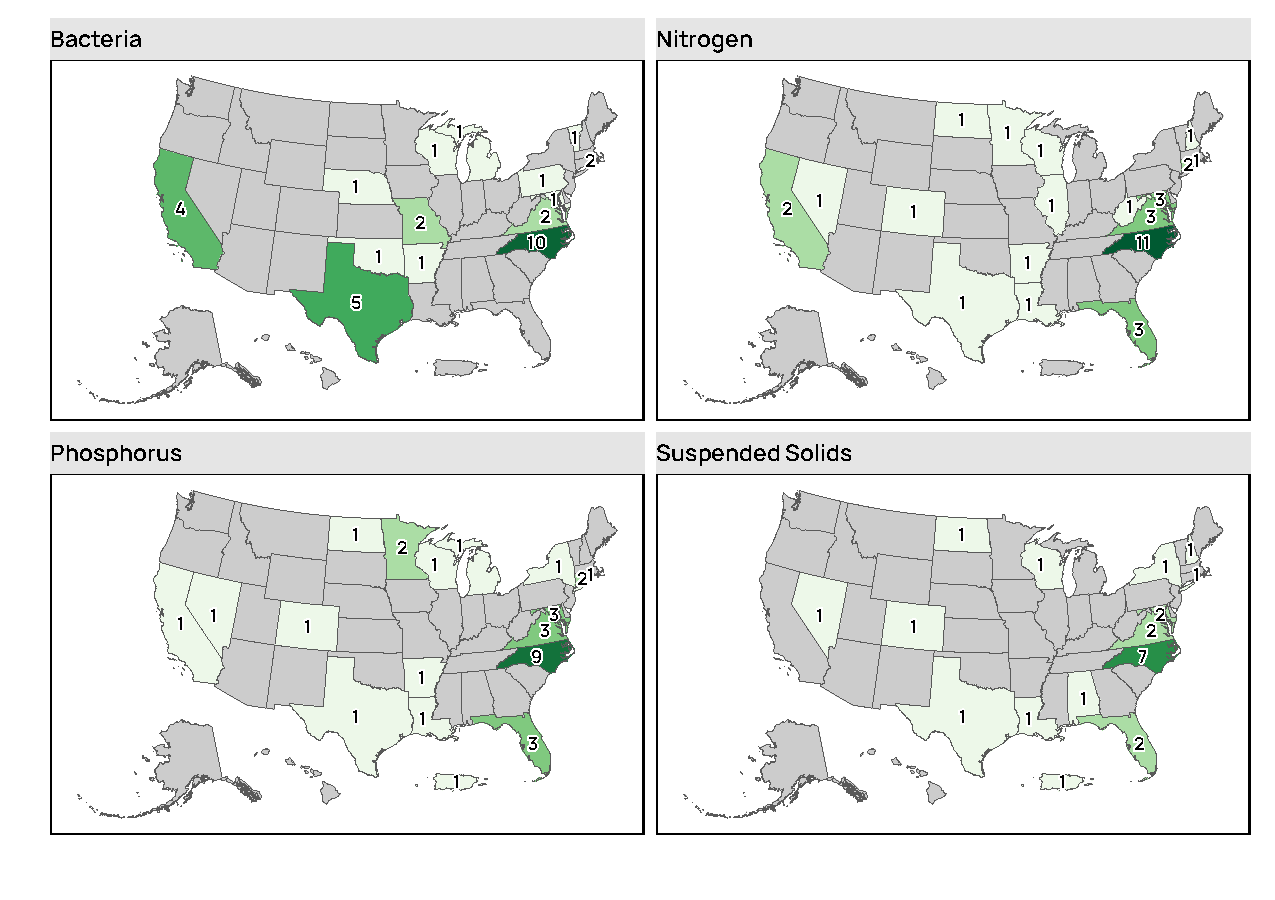
\includegraphics[width=1\linewidth,]{../figures/study_map} \caption{Distribution of studies identified in the systematic review by state and parameter.}\label{fig:studymap}
\end{figure}

\begin{figure}
\includegraphics[width=1\linewidth,]{../figures/bmp_summary} \caption{Summary of (A) study scale, (B) dominant runoff source, and (C) BMPs identified in the systematic review.}\label{fig:bmpsummary}
\end{figure}

\begin{figure}[H]
\includegraphics[width=1\linewidth,]{../figures/overall_effect} \caption{Estimated effect sizes and intervals from the null multilevel random effects model. Individual points represent studies, with size scaled by sampling variance. The point estimate with uncertaintity bars indicate the estimated overall effect, 95\% confidence intervals, and 95\% prediction intervals. Here, \textit{k} indicates the number of overall effects with the number of unique studies in parenthesis.}\label{fig:overalleffect}
\end{figure}



\end{document}
